% Paper 1 -- main document. Introduction and Results 1 are drafted; later sections are stubs
% (their plan lives in schematic.tex). Every number in the text is a macro from numbers.tex,
% generated by ../1BQF_to_spectral_filter_corpus/13_paper_numbers.py.
\documentclass[11pt,a4paper]{article}
\usepackage[T1]{fontenc}\usepackage[utf8]{inputenc}\usepackage{lmodern}
\usepackage[margin=2.3cm]{geometry}
\usepackage{amsmath,amssymb}\usepackage{booktabs}\usepackage{graphicx}
\usepackage[labelfont=bf,font=small,skip=4pt]{caption}
\usepackage{subcaption}\usepackage{float}\usepackage{xcolor}
\usepackage{tikz}\usetikzlibrary{decorations.pathreplacing,calc}
% TikZ styles and helpers shared by figures/circuits.tex and figures/circuits_qsvt.tex
\tikzset{
  wire/.style={line width=0.55pt},
  gate/.style={draw,fill=white,minimum height=6.2mm,minimum width=7.5mm,inner sep=1.5pt,font=\small,line width=0.55pt},
  wgate/.style={gate,minimum width=13mm},
  ctrl/.style={circle,fill=black,inner sep=0pt,minimum size=1.9mm},
  octrl/.style={circle,draw,fill=white,inner sep=0pt,minimum size=1.9mm,line width=0.55pt},
  targ/.style={circle,draw,inner sep=0pt,minimum size=3.2mm,line width=0.55pt},
  meter/.style={draw,fill=white,minimum height=6.2mm,minimum width=7.5mm,line width=0.55pt},
  reg/.style={font=\small,anchor=east},
  blk/.style={font=\footnotesize,anchor=north,text=black!65},
  st/.style={font=\footnotesize,anchor=south,text=blue!45!black},
  brace/.style={decorate,decoration={brace,mirror,amplitude=2.2pt},line width=0.4pt,black!60},
  slash/.style={},
}
\newcommand{\slashwire}[3]{% x y label : the /n mark on a multi-qubit wire
  \draw[line width=0.7pt] (#1cm-1.3mm,#2cm-1.6mm) -- (#1cm+1.3mm,#2cm+1.6mm);
  \node[font=\scriptsize,anchor=south west,inner sep=0.4pt] at (#1cm+0.9mm,#2cm+0.9mm) {#3};}
\newcommand{\vsep}[3]{% x ybot ytop : a dashed block boundary
  \draw[dashed,black!45,line width=0.4pt] (#1cm,#2cm) -- (#1cm,#3cm);}


\usepackage{microtype}
\usepackage[colorlinks=true,linkcolor=blue!60!black,citecolor=green!45!black,urlcolor=blue!70!black]{hyperref}
\usepackage[numbers,sort&compress]{natbib}
\graphicspath{{figures/}}
% Generated by 1BQF_to_spectral_filter_corpus/13_paper_numbers.py -- do not edit by hand.
\newcommand{\NEvents}{10}
\newcommand{\NEventsTotal}{80}
\newcommand{\HitLossMean}{1.0}
\newcommand{\HitLossMin}{0.5}
\newcommand{\HitLossMax}{1.8}
\newcommand{\SigmaPMeas}{0.39}
\newcommand{\SigmaPPred}{0.40}
\newcommand{\CheckMaxDiff}{1e-7}
\newcommand{\EpsMrad}{1.70}
\newcommand{\EpsCos}{1.44\times10^{-6}}
\newcommand{\ResidualRms}{4.8}
\newcommand{\TrueOutside}{8.6\times10^{-5}}
\newcommand{\ClassFarTwoHundred}{0.12}
\newcommand{\OneBitFarTwoHundred}{0.12}
\newcommand{\QsvtEffTwoHundred}{0.984}
\newcommand{\QsvtEffMinTwoHundred}{0.969}
\newcommand{\QsvtFarTwoHundred}{0.56}
\newcommand{\ClassEffAtOneTwoHundred}{0.98}
\newcommand{\OneBitEffAtOneTwoHundred}{0.98}
\newcommand{\ClassFarFourHundred}{0.35}
\newcommand{\OneBitFarFourHundred}{0.35}
\newcommand{\QsvtEffFourHundred}{0.973}
\newcommand{\QsvtEffMinFourHundred}{0.938}
\newcommand{\QsvtFarFourHundred}{0.36}
\newcommand{\ClassEffAtOneFourHundred}{0.97}
\newcommand{\OneBitEffAtOneFourHundred}{0.49}
\newcommand{\ClassFarSevenHundred}{0.63}
\newcommand{\OneBitFarSevenHundred}{0.63}
\newcommand{\QsvtEffSevenHundred}{0.937}
\newcommand{\QsvtEffMinSevenHundred}{0.919}
\newcommand{\QsvtFarSevenHundred}{1.00}
\newcommand{\ClassEffAtOneSevenHundred}{0.49}
\newcommand{\OneBitEffAtOneSevenHundred}{0.49}
\newcommand{\ClassFarThousand}{0.77}
\newcommand{\OneBitFarThousand}{0.77}
\newcommand{\QsvtEffThousand}{0.917}
\newcommand{\QsvtEffMinThousand}{0.893}
\newcommand{\QsvtFarThousand}{1.00}
\newcommand{\ClassEffAtOneThousand}{0.24}
\newcommand{\OneBitEffAtOneThousand}{0.49}
\newcommand{\KeptPair}{0.38}
\newcommand{\KeptTriple}{0.53}
\newcommand{\KeptTrack}{0.59}
\newcommand{\KeptHubThree}{0.63}
\newcommand{\KeptHubFive}{0.77}
\newcommand{\AtlasPairs}{127{,}816}
\newcommand{\AtlasPairsKeptClass}{127{,}816}
\newcommand{\AtlasPairsKeptQsvt}{0}
\newcommand{\AtlasTriples}{5{,}074}
\newcommand{\AtlasTriplesKeptQsvt}{87}
\newcommand{\AtlasComplete}{35{,}952}
\newcommand{\AtlasCompleteKeptQsvt}{35{,}952}
\newcommand{\AtlasBroken}{1{,}057}
\newcommand{\AtlasBrokenLostQsvt}{1{,}057}
\newcommand{\AtlasContamLostQsvt}{2{,}222}
\newcommand{\IsolatedShare}{99.7}
\newcommand{\AtlasQsvtEff}{0.916}
\newcommand{\AtlasQsvtFar}{0.005}
\newcommand{\AtlasClassFar}{0.77}
\newcommand{\AtlasClassEff}{0.996}
\newcommand{\TrackInputWeightLow}{94.7}
\newcommand{\TrackSolutionWeightLow}{98.5}
\newcommand{\ContamNearTrue}{6}
\newcommand{\HubNearTrue}{88}
\newcommand{\TripleNearTrue}{0.7}
\newcommand{\QTrackLow}{0.995}
\newcommand{\QTrackHigh}{0.526}
\newcommand{\QIso}{0.007}
\newcommand{\QPairLow}{0.014}
\newcommand{\QPairHigh}{0.044}
\newcommand{\QTripleLow}{0.439}
\newcommand{\QTripleHigh}{0.198}
\newcommand{\QHubLow}{0.846}
\newcommand{\QHubHigh}{0.374}
\newcommand{\PairSuppression}{45}
\newcommand{\DomainLow}{0.24}
\newcommand{\DomainHigh}{7.76}
\newcommand{\DomainHalfWidth}{3.76}
\newcommand{\DomainLength}{7.52}
\newcommand{\ResolutionForty}{0.19}
\newcommand{\ResolutionSixty}{0.13}
\newcommand{\NIsolatedThousand}{39{,}077{,}686}
\newcommand{\TeethFourSeven}{0.935}
\newcommand{\TeethFourThousand}{0.928}
\newcommand{\TeethBrightThousand}{0.925}
\newcommand{\TeethDarkTwoHundred}{0.014}
\newcommand{\TeethDarkThousand}{0.000}
\newcommand{\TeethBestSeven}{0.960}
\newcommand{\TeethBestThousand}{0.951}
\newcommand{\TeethFourSixtySeven}{0.960}
\newcommand{\TeethFourSixtyThousand}{0.937}
\newcommand{\TeethNDesigns}{25}
\newcommand{\ClassCloseUpToT}{400}
\newcommand{\ClassDropT}{700}
\newcommand{\OneBitPlateau}{0.49}
\newcommand{\NSysFourHundred}{20}
\newcommand{\CxEvoFourHundred}{6.2\times10^{5}}
\newcommand{\CxHitFourHundred}{1.7\times10^{4}}
\newcommand{\WidthOneBitFourHundred}{22}
\newcommand{\POneBitFourHundred}{1.0\times10^{-3}}
\newcommand{\RoundsOneBitFourHundred}{24}
\newcommand{\TotalCallsOneBitFourHundred}{49}
\newcommand{\GatesEvoOneBitFourHundred}{3.0\times10^{7}}
\newcommand{\GatesHitOneBitFourHundred}{8.1\times10^{5}}
\newcommand{\WidthPhaseFourHundred}{24}
\newcommand{\PPhaseFourHundred}{4.1\times10^{-4}}
\newcommand{\RoundsPhaseFourHundred}{39}
\newcommand{\TotalCallsPhaseFourHundred}{6171}
\newcommand{\GatesEvoPhaseFourHundred}{3.8\times10^{9}}
\newcommand{\GatesHitPhaseFourHundred}{1.0\times10^{8}}
\newcommand{\WidthWalkFourHundred}{27}
\newcommand{\PWalkFourHundred}{1.1\times10^{-3}}
\newcommand{\RoundsWalkFourHundred}{24}
\newcommand{\TotalCallsWalkFourHundred}{1492}
\newcommand{\GatesEvoWalkFourHundred}{9.3\times10^{8}}
\newcommand{\GatesHitWalkFourHundred}{2.5\times10^{7}}
\newcommand{\WidthHhlFourHundred}{29}
\newcommand{\PHhlFourHundred}{1.3\times10^{-1}}
\newcommand{\RoundsHhlFourHundred}{2}
\newcommand{\TotalCallsHhlFourHundred}{1116}
\newcommand{\GatesEvoHhlFourHundred}{6.9\times10^{8}}
\newcommand{\GatesHitHhlFourHundred}{1.9\times10^{7}}
\newcommand{\NSysThousand}{22}
\newcommand{\CxEvoThousand}{2.0\times10^{6}}
\newcommand{\CxHitThousand}{3.6\times10^{4}}
\newcommand{\WidthOneBitThousand}{24}
\newcommand{\POneBitThousand}{8.6\times10^{-4}}
\newcommand{\RoundsOneBitThousand}{27}
\newcommand{\TotalCallsOneBitThousand}{54}
\newcommand{\GatesEvoOneBitThousand}{1.1\times10^{8}}
\newcommand{\GatesHitOneBitThousand}{1.9\times10^{6}}
\newcommand{\WidthPhaseThousand}{26}
\newcommand{\PPhaseThousand}{2.3\times10^{-4}}
\newcommand{\RoundsPhaseThousand}{52}
\newcommand{\TotalCallsPhaseThousand}{8315}
\newcommand{\GatesEvoPhaseThousand}{1.6\times10^{10}}
\newcommand{\GatesHitPhaseThousand}{3.0\times10^{8}}
\newcommand{\WidthWalkThousand}{29}
\newcommand{\PWalkThousand}{7.3\times10^{-4}}
\newcommand{\RoundsWalkThousand}{29}
\newcommand{\TotalCallsWalkThousand}{1838}
\newcommand{\GatesEvoWalkThousand}{3.6\times10^{9}}
\newcommand{\GatesHitWalkThousand}{6.6\times10^{7}}
\newcommand{\WidthHhlThousand}{31}
\newcommand{\PHhlThousand}{7.1\times10^{-2}}
\newcommand{\RoundsHhlThousand}{3}
\newcommand{\TotalCallsHhlThousand}{1499}
\newcommand{\GatesEvoHhlThousand}{3.0\times10^{9}}
\newcommand{\GatesHitHhlThousand}{5.4\times10^{7}}
\newcommand{\CallsOneBit}{2}
\newcommand{\CallsPhase}{160}
\newcommand{\CallsWalk}{63}
\newcommand{\CallsHhl}{510}
\newcommand{\PPhasePrefactor}{0.05}
\newcommand{\PPhaseExponent}{0.77}
\newcommand{\POneBitPrefactor}{0.05}
\newcommand{\POneBitExponent}{0.61}
\newcommand{\CxEvoPrefactor}{152}
\newcommand{\CxEvoExponent}{1.37}
\newcommand{\CxHitPrefactor}{103}
\newcommand{\CxHitExponent}{0.85}
\newcommand{\MeasuredTMax}{400}
\newcommand{\HitOracleAncillas}{45}
\newcommand{\ScanNEvents}{2}
\newcommand{\ScanClassTenUmTwoHundred}{0.25}
\newcommand{\ScanOneBitTenUmTwoHundred}{0.25}
\newcommand{\ScanQsvtTenUmTwoHundred}{0.94}
\newcommand{\ScanClassTenUmFourHundred}{0.49}
\newcommand{\ScanOneBitTenUmFourHundred}{0.49}
\newcommand{\ScanQsvtTenUmFourHundred}{0.90}
\newcommand{\ScanClassTenUmSevenHundred}{0.00}
\newcommand{\ScanOneBitTenUmSevenHundred}{0.00}
\newcommand{\ScanQsvtTenUmSevenHundred}{0.00}
\newcommand{\ScanClassTenUmThousand}{0.00}
\newcommand{\ScanOneBitTenUmThousand}{0.00}
\newcommand{\ScanQsvtTenUmThousand}{0.00}
\newcommand{\ScanClassFifteenUmTwoHundred}{0.33}
\newcommand{\ScanOneBitFifteenUmTwoHundred}{0.34}
\newcommand{\ScanQsvtFifteenUmTwoHundred}{0.57}
\newcommand{\ScanClassFifteenUmFourHundred}{0.00}
\newcommand{\ScanOneBitFifteenUmFourHundred}{0.12}
\newcommand{\ScanQsvtFifteenUmFourHundred}{0.47}
\newcommand{\ScanClassFifteenUmSevenHundred}{0.00}
\newcommand{\ScanOneBitFifteenUmSevenHundred}{0.00}
\newcommand{\ScanQsvtFifteenUmSevenHundred}{0.22}
\newcommand{\ScanClassFifteenUmThousand}{0.00}
\newcommand{\ScanOneBitFifteenUmThousand}{0.00}
\newcommand{\ScanQsvtFifteenUmThousand}{0.00}
\newcommand{\ScanClassThreeUmTwoHundred}{0.99}
\newcommand{\ScanOneBitThreeUmTwoHundred}{0.99}
\newcommand{\ScanQsvtThreeUmTwoHundred}{0.99}
\newcommand{\ScanClassThreeUmFourHundred}{0.98}
\newcommand{\ScanOneBitThreeUmFourHundred}{0.98}
\newcommand{\ScanQsvtThreeUmFourHundred}{0.98}
\newcommand{\ScanClassThreeUmSevenHundred}{0.98}
\newcommand{\ScanOneBitThreeUmSevenHundred}{0.74}
\newcommand{\ScanQsvtThreeUmSevenHundred}{0.98}
\newcommand{\ScanClassThreeUmThousand}{0.24}
\newcommand{\ScanOneBitThreeUmThousand}{0.24}
\newcommand{\ScanQsvtThreeUmThousand}{0.95}
\newcommand{\ScanClassFiveUmTwoHundred}{0.50}
\newcommand{\ScanOneBitFiveUmTwoHundred}{0.50}
\newcommand{\ScanQsvtFiveUmTwoHundred}{0.99}
\newcommand{\ScanClassFiveUmFourHundred}{0.98}
\newcommand{\ScanOneBitFiveUmFourHundred}{0.74}
\newcommand{\ScanQsvtFiveUmFourHundred}{0.98}
\newcommand{\ScanClassFiveUmSevenHundred}{0.24}
\newcommand{\ScanOneBitFiveUmSevenHundred}{0.49}
\newcommand{\ScanQsvtFiveUmSevenHundred}{0.94}
\newcommand{\ScanClassFiveUmThousand}{0.00}
\newcommand{\ScanOneBitFiveUmThousand}{0.25}
\newcommand{\ScanQsvtFiveUmThousand}{0.92}
\newcommand{\SegClassTau}{0.35}
\newcommand{\SegFarClassThousand}{0.13}
\newcommand{\SegFarOneBitThousand}{0.77}
\newcommand{\SegFarQsvtThousand}{0.39}
\newcommand{\CircuitCheckT}{3}
\newcommand{\CircuitCheckLo}{0.2}
\newcommand{\CircuitCheckHi}{7.8}
\newcommand{\CircuitCheckNSeg}{36}
\newcommand{\CircuitCheckErrEven}{2.2\times10^{-9}}
\newcommand{\CircuitCheckErrOdd}{1.6\times10^{-7}}
\newcommand{\PruneKeptFourHundred}{2{,}402}
\newcommand{\PruneQubitsFullFourHundred}{20}
\newcommand{\PruneQubitsFourHundred}{12}
\newcommand{\PruneQubitsThreeFourHundred}{11}
\newcommand{\PrunePGainFourHundred}{258}
\newcommand{\PruneRoundsGainFourHundred}{16}
\newcommand{\PruneOneBitEffFourHundred}{0.97}
\newcommand{\PruneOneBitT}{1.15}
\newcommand{\PruneKeptThousand}{17{,}092}
\newcommand{\PruneQubitsFullThousand}{22}
\newcommand{\PruneQubitsThousand}{15}
\newcommand{\PruneQubitsThreeThousand}{13}
\newcommand{\PrunePGainThousand}{224}
\newcommand{\PruneRoundsGainThousand}{15}
\newcommand{\PruneOneBitEffThousand}{0.49}
\newcommand{\PruneMinDegreeThousand}{20}

\newcommand{\eff}{\ensuremath{\varepsilon_{\rm seg}}}
\newcommand{\far}{\ensuremath{f_{\rm seg}}}
\makeatletter
\newlabel{fig:circuits}{{2}{}{}{}{}}
\newlabel{sec:fork:trotter}{{Methods}{}{}{}{}}
\makeatother

% Review mark-up (Oct 2026): JS = J. Schuetz (blue), MM = M. Merk (purple), GS = G. Scriven's replies (dark orange).
\newcommand{\js}[1]{{\color{blue} JS: #1 }}
\newcommand{\mm}[1]{{\color{purple} MM: #1 }}
\newcommand{\gs}[1]{{\color{orange!85!black} GS: #1 }}
\newcommand{\R}{\mathbb{R}}

\title{From one bit to any polynomial:\\ quantum spectral filters for track finding in the LHCb vertex detector}
\author{G.\,W.\,Scriven, X.\,Chiotopoulos, D.\,Nicotra, J.\,Sch\"utz, J.\,de\,Vries, M.\,Merk\\
\small (author list and affiliations to be agreed)}
\date{Draft, \today}

\begin{document}
\maketitle

\begin{abstract}
\noindent\textit{Draft, to be finalised with the results sections.}
The one-bit quantum filter reconstructs particle-track segments by applying one cosine of a
segment Hamiltonian, which removes the isolated false segments at a small fraction of the cost
of quantum phase estimation. On simulated events with detector noise it keeps a high
efficiency, but a false rate of $\OneBitFarFourHundred$ at 400 tracks and $\OneBitFarThousand$
at 1000. We show that the filter is the degree-one member of the polynomial transforms
provided by the quantum singular value transformation, and that a degree-40 polynomial on the
same Hamiltonian keeps $\QsvtEffThousand$ of true segments at a false rate below $1\%$ at 1000
tracks. We identify which configurations each filter keeps from their eigenvalues alone, and
give the cost of the polynomial in calls, gates and qubits.
\end{abstract}

\section{Introduction}


\mm{Added some explanatory text and connection to previous papers: whenever we use things like "isolated segments" they are not yet defined and not understood unless defined. Hence, I do think we need the schematic illustration added below....} \\
\mm{
The reconstruction of events in particle-physics experiments at the High-Luminosity Large Hadron Collider (HL-LHC) presents an increasingly demanding computational challenge. Charged-particle trajectory reconstruction, or tracking, is a central component of this problem: from a large collection of spatial measurements ("hits") recorded by the detector, the reconstruction algorithm must identify measurements originating from the same charged particle and determine the parameters of its trajectory. The strongly increasing particle multiplicities foreseen at the HL-LHC make this an increasingly challenging combinatorial pattern-recognition problem.
Track reconstruction provides an interesting use case for hybrid quantum--classical computing because the combinatorial problem can be mapped onto a linear-algebra problem. In our earlier work \cite{Nicotra}, following the Hamiltonian formulation introduced by Denby and Peterson \cite{Denby,Peterson}, the track-finding problem was expressed through the minimization of an Ising-like Hamiltonian, which was solved using the Harrow--Hassidim--Lloyd (HHL) quantum linear-systems algorithm. The resulting matrices were found to satisfy two important requirements for an efficient HHL implementation: increasing sparsity with problem size and a bounded condition number. Under these assumptions, HHL offers the prospect of an exponential improvement in the dependence on the dimension of the linear system. In practice, however, the circuit depth associated with high-precision quantum phase estimation and Hamiltonian simulation, together with the cost of extracting the solution from the quantum state, places it beyond near-term QPU hardware.
In subsequent work \cite{Chiotopoulos}, we found that 
a much reduced precision system, restricting the phase estimation to a single bit resulted in the 1-Bit Quantum Filter; a single-ancilla circuit that applies one cosine with its zero placed on the eigenvalue shared by every isolated false track segment, strongly reducing both circuit depth and the number of required readout samples.
The filter requires two calls to the time
evolution where phase estimation needs hundreds, it suppresses the bulk of the false candidates
before readout, and it was validated against the noise models of trapped-ion and superconducting QPU's. 
}

\mm{
The 1-Bit Quantum Filter nevertheless implements only a relatively simple spectral discrimination. At increasing track density, the spectrum contains more complicated structures associated with combinatorial track candidates, and a single spectral threshold is insufficient to suppress all classes of incorrectly reconstructed segments. This motivates replacing the binary spectral discriminator by a controllable higher-order spectral transformation.
In this work, we introduce such a generalization using Quantum Singular Value Transformation (QSVT). QSVT provides a systematic framework for implementing polynomial transformations of the spectrum of a suitably encoded Hamiltonian, thereby allowing the spectral response of the quantum filter to be engineered beyond a single threshold. Instead of merely separating one noise eigenspace from the remaining spectrum, the filter can be designed to selectively enhance spectral regions associated with physical track configurations while suppressing multiple classes of unwanted eigenstates. In this way, the 1-Bit Quantum Filter provides the conceptual starting point for a more general spectral-filtering approach, while QSVT supplies the mathematical framework required to construct and optimize the full filter developed in this work.}
\\[0.5cm]


At the High-Luminosity LHC a single bunch crossing will leave thousands of charged-particle
hits in the LHCb vertex detector, and the first step of reconstruction is to decide which hits
belong to the same particle. Between two detector planes with $T$ hits each there are $T^2$
candidate segments but only $T$ real ones, so the search for tracks is a search for a thin
signal in a background that grows quadratically with the number of particles. It is also one
of the few reconstruction tasks that can be written exactly as linear algebra. Denby and
Peterson cast track finding as the minimisation of a quadratic energy over candidate
segments~\cite{denby1988,peterson1989}; relaxing the segment variables to real numbers turns
that minimisation into a linear system whose solution scores every segment.

That observation started a short line of work on quantum algorithms for the problem. Nicotra
et al.\ solved the linear system with the Harrow--Hassidim--Lloyd algorithm~\cite{hhl2009} and
found tracking performance comparable to the classical solver, but a circuit whose depth, and
the number of samples needed to read out its answer, placed it far beyond near-term
hardware~\cite{nicotra2023}. Chiotopoulos et al.\ then observed that tracking does not need the
solution's precise values, only which segments are switched on. Restricting phase estimation
to a single bit~\cite{trackhhl_epj} became the one-bit quantum filter~\cite{trackhhl}: a
single-ancilla circuit that applies one cosine of the Hamiltonian, with its zero placed on the
eigenvalue shared by every isolated false segment. The filter needs two calls to the time
evolution where phase estimation needs hundreds, it suppresses the bulk of the false candidates
before readout, and it was validated against the noise models of trapped-ion and
superconducting processors~\cite{trackhhl}.

What the single zero leaves behind has not been measured. The one-bit filter was built to cut
the cost of reading out the answer, and it succeeds for the isolated false segments, which make
up $\IsolatedShare\%$ of all false candidates at 1000 tracks \js{Is this true in general? Or only for a toy problem?} \gs{This is a property of the geometry, not of the toy. Two planes with $T$ hits each give $T^2$ candidate segments. A false segment couples to a second segment only when a third hit lies inside the window $\theta_{\max}$ around its line. The number of such hits is proportional to the hit density times the window area. Thus the isolated share increases with $T$ at a fixed window. The value $\IsolatedShare\%$ is for this set of events. Our check on LHCb Run-3 data shows the same classes of false segments. We will add one sentence with this argument.}. The remainder are not isolated: accidental pairs,
triples and hubs of compatible false segments, each with its own eigenvalues. On events with
detector noise we find that the one-bit filter keeps the efficiency of the classical solver
but also its false segments: read where it keeps $99\%$ of true segments, its false rate is
$\OneBitFarFourHundred$ at 400 tracks and $\OneBitFarThousand$ at 1000. \js{Where are these numbers from? Cite or explain.} \gs{All numbers come from the one set of simulated events of section~\ref{sec:r1}. Each number in the text is a macro that the analysis script writes. We will add a forward reference to table~\ref{tab:headline} here.}

A cosine has one zero \js{A difficult statement for a mathematician ;-) Also, how is it connected to the rest?} \gs{Agreed. The sentence means: on the eigenvalue axis, the one-bit response $\cos(\lambda t/2)$ has one zero inside the spectrum of $A$. A QSVT response of degree $d$ has up to $d$ zeros. We will rewrite the sentence and make the link to the next sentence explicit.}. The quantum singular value
transformation~\cite{gslw2019,martyn2021} applies any polynomial bounded by 1 on $[-1,1]$ \js{there is no such thing as a bounded polynomial, save the constant} \gs{Corrected. The text now says `polynomial bounded by 1 on $[-1,1]$' at each occurrence. This is the condition of the QSVT theorem.} of a Hamiltonian at a
cost linear in its degree, and the one-bit filter is its degree-one member. In this paper we
use that freedom. We show that the true tracks of the detector occupy a small set of known
eigenvalues, that a polynomial passing those eigenvalues and rejecting the rest keeps a
comparable efficiency ($\QsvtEffThousand$ at 1000 tracks) while cutting the false rate below
$1\%$, and we identify exactly which configurations each filter keeps and why. The price is a
deeper circuit and, for the block encoding that makes it efficient, more qubits; we give both.

Section~\ref{sec:r1} builds the problem from a noisy event: the detector model, the acceptance
window, the Hamiltonian, the one-bit filter, and what each solver keeps.
\textit{[Sections on the spectrum, the polynomial, results against multiplicity and cost follow;
see schematic.tex.]}

\section{Results}
\js{Seems a bit odd to me to start with results. Why do you not start with a description of the methodology?} \gs{This is the format of Communications Physics: Introduction, Results, Discussion, Methods. This journal published the one-bit filter paper, and we target it again. We keep this format. The detector, window and Hamiltonian paragraphs stay short here. The Methods section will give the full derivations.}
\subsection{From hits to a filter}\label{sec:r1}

\paragraph{The detector and its noise.}
We use the simplified vertex detector of refs.~\cite{nicotra2023,trackhhl}: five planes
$\Delta z=33$\,mm apart, $T$ tracks per event from a common vertex inside a cone of half-opening
$0.2$\,rad, and one hit per track on each plane (figure~\ref{fig:hits}a). Three detector effects
are applied throughout: Gaussian smearing of every hit with $\sigma_{\rm res}=5\,\mu$m, a
multiple-scattering kink of $\sigma_{\rm scatt}=0.15$\,mrad at every plane, which \js{which = ?} \gs{`which' refers to the scattering kink. A kink of $0.15$\,mrad per plane is the multiple-scattering angle of a track of high momentum in one silicon plane. We will rewrite the sentence.} corresponds
to an ideal high-momentum track, and the loss of $1\%$ of hits. Every result in this paper is
computed on one set of events at this configuration, $\NEvents$ events for each of
$T=10,20,50,100,200,400,700$ and $1000$ tracks; on them the measured hit residuals are
$\ResidualRms\,\mu$m and the hit loss is $\HitLossMean\%$ on average. \js{I am not sure all these numbers should be placed here. In a numerical mathematics paper: Intro, Methodology, Numerical Results, Conclusion} \gs{In the Communications Physics format the Results section states the data configuration once. We will keep only the configuration here and move the measured residual and the measured hit loss to Methods.}

\paragraph{The acceptance window.}
As in refs.~\cite{nicotra2023,trackhhl}, the candidate segments are doublets of hits on adjacent
planes, each described by a variable $S_i\in\{0,1\}$ \js{$1 \leq i \leq T$ (??)} \gs{No. The index $i$ runs over all candidate doublets, not over tracks. Five planes with $T$ hits each give $N=4T^2$ candidates, and $S\in\{0,1\}^N$. We will state $N$ at this point.}, and two segments $S_i$ and $S_j$ that share a
hit are coupled when the angle $\theta_{ij}$ between them passes an angular tolerance $\varepsilon$: \js{Stupid question, just for my understanding, shouldn't $S$ be indexed by $i$ and another index (call it $k$) that refers to the plane where it is measured? And then $\theta_{ij}$ is the angle between $S_i^k$ and $S_j^{k+1}$?} \gs{A segment is identified by its two hits, so the plane index is implicit: a segment joins plane $k$ to plane $k+1$. Two segments share a hit only when one ends on the plane where the other starts. We use one flat index $i$ because the matrix $A$ is indexed in this way. We will add one sentence that says this.}
\begin{equation} 
f(\theta_{ij},\varepsilon)=\begin{cases}1,&\cos\theta_{ij}\ge1-\varepsilon,\\0,&\text{otherwise}.\end{cases}
\end{equation}
We set the tolerance from the detector. Resolution and scattering give a true continuation \js{true continuation = straight line?} \gs{A true continuation is a pair of segments of the same track on planes $k$, $k+1$ and $k+2$. Without noise the pair is a straight line. With noise the second segment turns by a small kink angle. We will define the term at its first use.} a kink
whose projections \js{projections onto what?} \gs{The projections of the kink angle on the two transverse axes $x$ and $y$. Each projection is Gaussian with width $\sigma_p$.} are Gaussian of width
\begin{equation}
\sigma_p^2=\sigma_{\rm scatt}^2+6\,\big(\sigma_{\rm res}/\Delta z\big)^2 ,
\end{equation}
so its magnitude follows a Rayleigh distribution \js{This is because if two normally distributed quantities are measured in the Euclidean norm, then this is Rayleigh-distributed, right?} \gs{Yes. The kink magnitude is the Euclidean norm of two independent Gaussian components with the same width. This norm follows a Rayleigh distribution.}, and we accept kinks below
\begin{equation}
\theta_{\max}=3\sqrt2\,\sigma_p=\EpsMrad\ \text{mrad},\qquad \varepsilon=1-\cos\theta_{\max}=\EpsCos ,
\end{equation}
which loses a fraction $e^{-9}\approx1.2\times10^{-4}$ of true continuations at any noise level. \js{I cannot really follow. Is this physics magic? Or where does it come from? What is 'true continuations'?} \gs{No magic, two steps. First, the kink is the second difference of three hit positions divided by $\Delta z$. Three independent position errors of width $\sigma_{\rm res}$ give the second difference a variance of $(1+4+1)\,\sigma_{\rm res}^2=6\sigma_{\rm res}^2$. This is the factor 6. Second, the Rayleigh tail is $P(\theta>\theta_{\max})=\exp[-\theta_{\max}^2/(2\sigma_p^2)]$. With $\theta_{\max}=3\sqrt2\,\sigma_p$ the exponent is $-9$. A true continuation is defined in our reply above. We will add both steps to the text.}
On the events the measured kink width is $\SigmaPMeas$\,mrad against $\SigmaPPred$\,mrad
predicted, and a fraction $\TrueOutside$ of true continuations falls outside the window,
while the false candidates lie at kinks one to three orders of magnitude larger
(figure~\ref{fig:hits}b). \js{In my opinion, if you talk about results from a figure, start with mentioning the figure and then describing its results.} \gs{Agreed. We will name figure~\ref{fig:hits}b first and then state what it shows.}

\paragraph{The Hamiltonian.}
Track finding is the search for the ground state of the Hamiltonian of 
refs.~\cite{nicotra2023,trackhhl}, \js{If I understand it correctly, we go from segment to segment, right? So $S$ is a vector in $\R^T$ rather than $\R^{T^2}$} \gs{$S$ is a vector in $\R^N$ with $N\approx4T^2$, one entry per candidate segment. The Hamiltonian couples only segment pairs that share a hit, so the sum over $i,j$ runs over these pairs.} 
\begin{equation}
\mathcal{H}(S)=\mathcal{H}_{\rm ang}(S,\varepsilon)+\alpha\,\mathcal{H}_{\rm spec}(S)+\beta\,\mathcal{H}_{\rm gap}(S),
\end{equation}
\begin{equation}
\mathcal{H}_{\rm ang}(S,\varepsilon)=-\frac12\sum_{i,j}f(\theta_{ij},\varepsilon)\,S_iS_j,\qquad
\mathcal{H}_{\rm spec}(S)=\frac12\sum_i S_i^2,\qquad
\mathcal{H}_{\rm gap}(S)=\frac12\sum_i\big(1-S_i\big)^2 ,
\end{equation}
where the angular term rewards compatible continuations and the two regularisation terms keep
the problem well posed.\footnote{Ref.~\cite{trackhhl} writes $\mathcal{H}_{\rm spec}$ and
$\mathcal{H}_{\rm gap}$ without the factor $\frac12$; the factor, which its reference
implementation carries, is what gives the diagonal $\alpha+\beta$ and $\mathbf{b}=\beta\,\mathbf{1}$
stated there.} Relaxing $S_i$ to a real vector $\mathbf{x}$, the minimum is found by setting the
gradient to zero, \js{Technically, as long as $f$ is a nonlinear function (which in this description, it is) this is not a linear but a nonlinear algebra problem!} \gs{$f$ acts on the measured angles $\theta_{ij}$, not on the unknowns $S$. The angles are data and are fixed before the solve. The energy is quadratic in $S$, so its gradient is linear in $\mathbf{x}$. We will say this in the text.}
\begin{equation}
\label{eq:Axb}
\nabla_{\mathbf{x}}\mathcal{H}=A\mathbf{x}-\mathbf{b}=0,\qquad A=(\alpha+\beta)\,I-C,\qquad \mathbf{b}=\beta\,\mathbf{1},
\end{equation}
\js{Should we define $\mathbf{1}$?} \gs{Yes. $\mathbf{1}$ is the vector of $N$ ones. We will define it at this equation.}
where $C_{ij}=f(\theta_{ij},\varepsilon)$ for segments that share a hit. We take $\alpha=3$ and
$\beta=1$, so every diagonal entry of $A$ is $\lambda_c=\alpha+\beta=4$ (ref.~\cite{trackhhl} used
$\alpha=2$, $\lambda_c=3$). Because compatibility is local, $A$ breaks into small blocks, one for
each connected group of compatible segments (figure~\ref{fig:hits}c \js{Maybe explain the figure just in one or two sentences, this would also simplify understanding the numbers below. Also explain that the figure only covers four tracks I guess ?!} \gs{Figure~\ref{fig:hits}c shows four connected groups cut from one 400-track event, not four tracks: a complete track (four segments in a chain), a false pair, a hub and an isolated false segment. Each group is one block of $A$. We will add this description to the text.}), and the solution on each
block depends only on its graph. \js{In this example, a} \gs{Accepted. The values below are exact for the graphs of figure~\ref{fig:hits}c, and they hold for every block with the same graph.} segment with no compatible neighbour solves to
$\beta/\lambda_c=(1/4)$; a complete five-hit track to $(4/11, 5/11, 5/11, 4/11)$; and a pair of compatible segments to $(1/3, 1/3)$, whether it is a genuine fragment of a track
that lost a hit or two false segments that happen to line up. Read at the threshold that keeps
$99\%$ of true segments, the classical solution admits a false rate of $\ClassFarFourHundred$ at
400 tracks (figure~\ref{fig:hits}d \js{How do I read this from the figure? I really don't like just pointing to figures and then leaving the reader alone with it. } \gs{Figure~\ref{fig:hits}d shows the histogram of the classical values $x_i$ on one 400-track event, true segments in green and false segments in red, with the threshold as a dashed line. The false rate is the red count to the right of the line divided by the total count to the right of the line. We will state this in the text.}): the threshold must reach down to the fragments at $1/3$, and
the false pairs share that level.
\js{We do not talk here AT ALL about eigenvalues, but they are way more important to the discussion, right? Would it not be a good idea to add eigenvalues here, and not talk about individual results?} \gs{Agreed. We will move the block spectrum (the first paragraph of section~\ref{sec:r2}) to this point and give the values $1/4$, $1/3$, $4/11$ and $5/11$ through the eigenvalues and eigenvectors of each block.} 


\begin{figure}[H]\centering
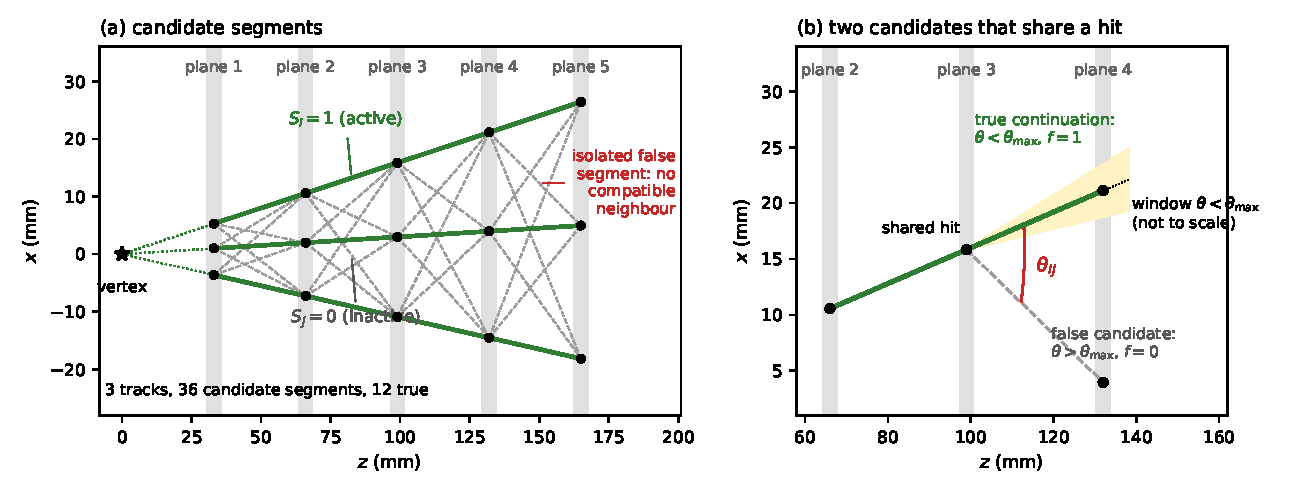
\includegraphics[width=0.95\textwidth]{fig0_toy_scheme.pdf}
\caption{\textbf{Candidate segments in a small event.} (a)~Three straight tracks from one vertex
cross five planes. Each pair of hits on adjacent planes is a candidate segment. The segments of the
true tracks are active ($S_i=1$, green). All other candidates are inactive ($S_j=0$, grey). In this
event no false candidate has a compatible neighbour, so each false candidate is an isolated false
segment. (b)~Two candidates that share one hit. The angle $\theta_{ij}$ between them is the kink.
The two segments are compatible ($f=1$) when the kink is smaller than $\theta_{\max}$. The window is
drawn much wider than the real $\theta_{\max}=\EpsMrad$\,mrad.}
\label{Fig:ToyEvent}
\end{figure}


\begin{figure}[t]
\centering
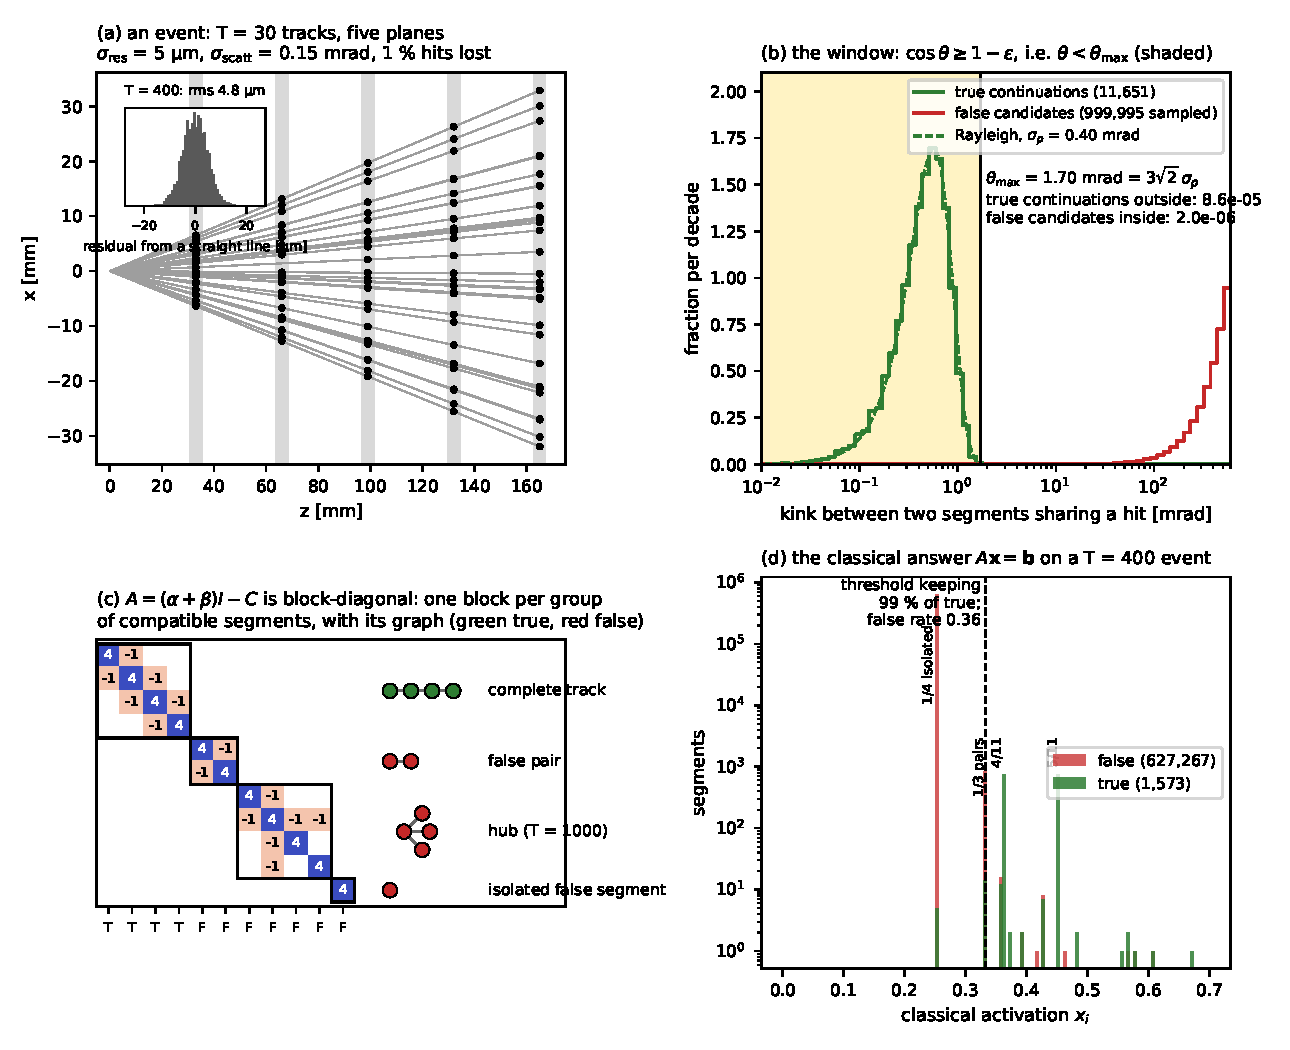
\includegraphics[width=\textwidth]{fig1_hits_to_hamiltonian.pdf}
\caption{\textbf{From hits to a Hamiltonian.} (a)~An event with $T=30$ tracks; inset, hit
residuals \js{what is this?} \gs{The hit residual is the distance in $x$ between a hit and the straight line fitted through all hits of its track. Its spread measures the resolution. We will define it in the caption.} from straight-line fits on a 400-track event. (b)~Kinks between segments that share a
hit: true continuations follow the Rayleigh law of width $\sigma_p$; false candidates lie far
outside the window $\theta<\theta_{\max}$ (shaded). (c)~Real blocks of $A=(\alpha+\beta)I-C$ and their graphs: a
complete track, a false pair, a hub and an isolated false segment. (d)~Classical activations on
a 400-track event with the threshold that keeps $99\%$ of true segments.}
\label{fig:hits}
\end{figure}

\paragraph{The one-bit filter.}
The one-bit filter (figure~\ref{fig:filters}a) prepares the uniform superposition over segments,
applies one bit of phase estimation to $e^{-iAt}$ with the phase bit $T$, sets the flag qubit $A$ when
$T$ reads zero, and uncomputes the phase bit. The $A=1$ part of the final state $|\Psi_4\rangle$ of
figure~\ref{fig:filters}a is \js{$\cos(A)$ is not meaningful in this context. It is a probability, so it should be scalar. And what is $\mathbf{u}$? I need a bit more context to follow. Maybe we can write up the outcome of the 1-bit filter, which should be something like } \gs{Agreed, and we have rewritten this part. $|u\rangle$ is the uniform state over the $N$ candidate segments, $\mathbf{u}$ its vector of amplitudes $u_i=1/\sqrt N$. $p_i$ is a scalar: $[\cdot]_i$ takes component $i$ of the vector in the brackets. The state you wrote is not the state the circuit makes. After the first round, the phase bit $T$ holds $|0\rangle_T\otimes e^{-iAt/2}\cos(At/2)|u\rangle-i\,|1\rangle_T\otimes e^{-iAt/2}\sin(At/2)|u\rangle$. The flag $A$ is set to 1 on the $T=0$ part. The uncompute then gives the state in the equation below, and this state gives $p_i$. We will write the state after each stage of figure~\ref{fig:filters}a in Methods.}
\begin{equation}
|1\rangle_A\otimes\Big[|0\rangle_T\otimes\cos^{2}\!\big(\tfrac{At}{2}\big)|u\rangle\;-\;\tfrac{i}{2}\,|1\rangle_T\otimes\sin(At)\,|u\rangle\Big],
\qquad |u\rangle=\frac{1}{\sqrt N}\sum_{i=1}^{N}|i\rangle ,
\end{equation}
where $N$ is the number of candidate segments, so that after post-selection on $A=1$ the
probability of reading segment $i$ is

\js{with $\psi = \frac 1 {2^n} \sum_{i=0}^{2^n-1} i$ and then continue from there? We could also clarify that $T = 2^n$ ?} \gs{The segment register has $n=\lceil\log_2 N\rceil$ qubits, with $N$ the number of candidate segments. $N$ is not a power of two in general. We will state $n$ at the register in figure~\ref{fig:filters}a and say in Methods how the unused basis states are treated.}
\begin{equation}
p_i=\Big[\cos^{2}\!\big(\tfrac{At}{2}\big)\mathbf{u}\Big]_i^{2}+\Big[\tfrac12\sin(At)\,\mathbf{u}\Big]_i^{2},\qquad t=\frac{\pi}{\lambda_c},
\end{equation}
\js{Btw, this should be the probability when the ancilla is zero, but in the plot it says it should be one.} \gs{Both are correct. The circuit has two ancillas. The phase bit $T$ returns to 0. The flag $A$ is set to 1 when $T=0$ after the first round, and the post-selection reads $A=1$. The text now names both registers.}
so the amplitude of every eigencomponent of the input is multiplied by $\cos(\lambda t/2)$ \js{should it not be the square?} \gs{The amplitude factor is $\cos(\lambda t/2)$. The probability weight is its square. The sentence now says `amplitude'.}. With $t=\pi/\lambda_c$ the
zero lands on $\lambda=\lambda_c$, the eigenvalue of every isolated segment \js{what about the $\sin$ contribution in $p_i$?} \gs{The sine term is the $T=1$ part of the same flagged state. Its amplitude on one eigencomponent is $\cos(\lambda t/2)\sin(\lambda t/2)$. It contains the factor $\cos(\lambda t/2)$, so it is also zero at $\lambda=\lambda_c$. The sum of the two terms on one eigencomponent is $\cos^2(\lambda t/2)$.}, and those segments are removed
exactly. Every other configuration keeps a factor fixed by where its eigenvalues lie
(figure~\ref{fig:filters}c): a false pair keeps $\KeptPair$, a false triple $\KeptTriple$, a
hub with three or five prongs $\KeptHubThree$ or $\KeptHubFive$, and a complete track
$\KeptTrack$ on the eigenvalue that carries almost all of its weight. Every hub keeps more of
itself than a real track does. Holding $99\%$ of true segments, the filter's threshold must again reach the fragments of
broken tracks, and the false pairs, triples and hubs above them all survive: on the median event its
false rate matches the classical one, $\OneBitFarFourHundred$ at 400 tracks,
$\OneBitFarSevenHundred$ at 700 and $\OneBitFarThousand$ at 1000.

\begin{figure}[p]
\centering
\resizebox{0.95\textwidth}{!}{% Figure 2 of paper 1 (16 Sep 2026): the one-bit filter, and the QSVT with the dilation encoding.
% Built from circuits.tex panel (b) and circuits_qsvt.tex panel (a); requires circuit_styles.tex.
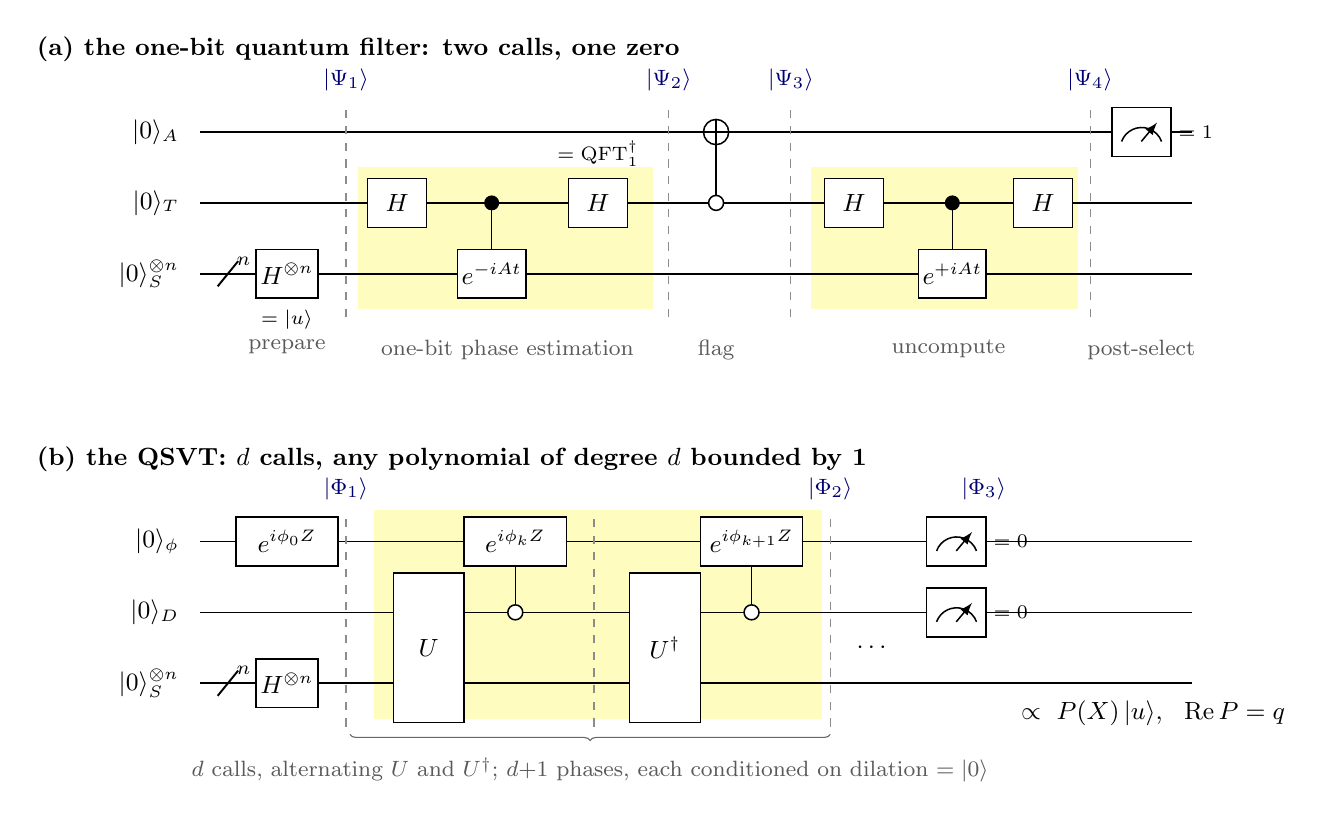
\begin{tikzpicture}[x=1cm,y=1cm]
\begin{scope}[shift={(0,0)}]
\fill[yellow!25] (2.0,-1.35) rectangle (5.75,0.45); \fill[yellow!25] (7.75,-1.35) rectangle (11.15,0.45);
\node[anchor=west,font=\small\bfseries] at (-2.2,1.95) {(a) the one-bit quantum filter: two calls, one zero};
\node[reg] at (-0.15,0.9)  {$|0\rangle_{A}$};
\node[reg] at (-0.15,0)    {$|0\rangle_{T}$};
\node[reg] at (-0.15,-0.9) {$|0\rangle^{\otimes n}_{S}$};
\draw[wire] (0,0.9) -- (12.6,0.9); \draw[wire] (0,0) -- (12.6,0); \draw[wire] (0,-0.9) -- (12.6,-0.9);
\slashwire{0.35}{-0.9}{$n$}
\node[gate] at (1.1,-0.9) {$H^{\otimes n}$};
\node[font=\scriptsize,anchor=north] at (1.1,-1.24) {$=|u\rangle$};
\vsep{1.85}{-1.45}{1.25}
\node[gate] at (2.5,0) {$H$};
\node[ctrl] at (3.7,0) {}; \draw[wire] (3.7,0) -- (3.7,-0.9); \node[gate] at (3.7,-0.9) {$e^{-iAt}$};
\node[gate] at (5.05,0) {$H$};
\node[font=\scriptsize,anchor=south] at (5.05,0.34) {$=\mathrm{QFT}_1^{\dagger}$};
\vsep{5.95}{-1.45}{1.25}
\node[octrl] at (6.55,0) {}; \draw[wire] (6.55,0.09) -- (6.55,0.9); \node[targ] at (6.55,0.9) {}; \draw[wire] (6.55,0.74) -- (6.55,1.06);
\vsep{7.5}{-1.45}{1.25}
\node[gate] at (8.3,0) {$H$};
\node[ctrl] at (9.55,0) {}; \draw[wire] (9.55,0) -- (9.55,-0.9); \node[gate] at (9.55,-0.9) {$e^{+iAt}$};
\node[gate] at (10.7,0) {$H$};
\vsep{11.3}{-1.45}{1.25}
\node[meter] at (11.95,0.9) {}; \draw[wire] (11.7,0.78) arc (160:20:0.27); \draw[wire,-latex] (11.95,0.78) -- (12.15,1.02);
\node[font=\scriptsize,anchor=west] at (12.3,0.9) {$=1$};
\node[blk] at (1.1,-1.62) {prepare};
\node[blk] at (3.9,-1.62) {one-bit phase estimation};
\node[blk] at (6.55,-1.62) {flag};
\node[blk] at (9.5,-1.62) {uncompute};
\node[blk] at (11.95,-1.62) {post-select};
\node[st] at (1.85,1.3) {$|\Psi_1\rangle$}; \node[st] at (5.95,1.3) {$|\Psi_2\rangle$};
\node[st] at (7.5,1.3) {$|\Psi_3\rangle$}; \node[st] at (11.3,1.3) {$|\Psi_4\rangle$};
\end{scope}
\begin{scope}[shift={(0,-5.2)}]
\fill[yellow!25] (2.2,-1.35) rectangle (7.9,1.3);
\node[anchor=west,font=\small\bfseries] at (-2.2,1.95) {(b) the QSVT: $d$ calls, any polynomial of degree $d$ bounded by 1};
\node[reg] at (-0.15,0.9)  {$|0\rangle_{\phi}$};
\node[reg] at (-0.15,0)    {$|0\rangle_{D}$};
\node[reg] at (-0.15,-0.9) {$|0\rangle^{\otimes n}_{S}$};
\draw[wire] (0,0.9) -- (12.6,0.9); \draw[wire] (0,0) -- (12.6,0); \draw[wire] (0,-0.9) -- (12.6,-0.9);
\slashwire{0.35}{-0.9}{$n$}
\node[gate] at (1.1,-0.9) {$H^{\otimes n}$};
\node[gate,minimum width=13mm] at (1.1,0.9) {$e^{i\phi_0 Z}$};
\vsep{1.85}{-1.45}{1.25}
% one repetition: U on (D,S), then the projector-controlled phase on the signal qubit
\node[gate,minimum height=19mm,minimum width=9mm] at (2.9,-0.45) {$U$};
\node[octrl] at (4.0,0) {}; \draw[wire] (4.0,0.09) -- (4.0,0.62);
\node[gate,minimum width=13mm] at (4.0,0.9) {$e^{i\phi_k Z}$};
\vsep{5.0}{-1.45}{1.25}
\node[gate,minimum height=19mm,minimum width=9mm] at (5.9,-0.45) {$U^{\dagger}$};
\node[octrl] at (7.0,0) {}; \draw[wire] (7.0,0.09) -- (7.0,0.62);
\node[gate,minimum width=13mm] at (7.0,0.9) {$e^{i\phi_{k+1} Z}$};
\vsep{8.0}{-1.45}{1.25}
\node[font=\small] at (8.55,-0.45) {$\cdots$};
\draw[brace] (1.9,-1.55) -- (8.0,-1.55); \node[blk] at (4.95,-1.72) {$d$ calls, alternating $U$ and $U^{\dagger}$; $d{+}1$ phases, each conditioned on dilation $=|0\rangle$};
\node[meter] at (9.6,0.9) {}; \draw[wire] (9.35,0.78) arc (160:20:0.27); \draw[wire,-latex] (9.6,0.78) -- (9.8,1.02);
\node[font=\scriptsize,anchor=west] at (9.95,0.9) {$=0$};
\node[meter] at (9.6,0) {}; \draw[wire] (9.35,-0.12) arc (160:20:0.27); \draw[wire,-latex] (9.6,-0.12) -- (9.8,0.12);
\node[font=\scriptsize,anchor=west] at (9.95,0) {$=0$};
\node[font=\small,anchor=north west] at (10.3,-1.0) {$\propto\ P(X)\,|u\rangle,\ \ \mathrm{Re}\,P=q$};
\node[st] at (1.85,1.3) {$|\Phi_1\rangle$}; \node[st] at (8.0,1.3) {$|\Phi_2\rangle$}; \node[st] at (9.95,1.3) {$|\Phi_3\rangle$};
\end{scope}
\end{tikzpicture}
}\\[6pt]
\begin{minipage}{0.70\textwidth}\centering
{\small\bfseries (c)}\\
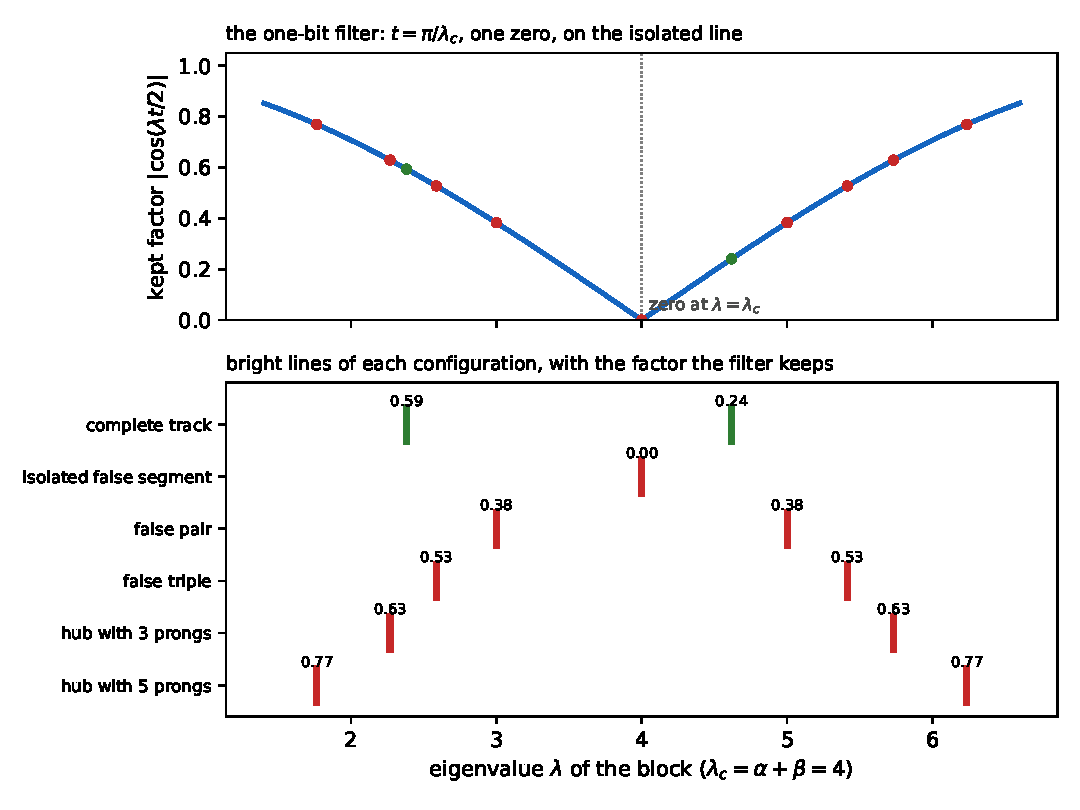
\includegraphics[width=\textwidth]{fig2_onebit_response.pdf}
\end{minipage}
\caption{\textbf{One zero, and any polynomial.} (a)~The one-bit filter: one bit of phase
estimation with two calls to the controlled evolution (highlighted) applies $\cos(\lambda t/2)$,
with a single zero at $\lambda=\lambda_c$. (b)~The quantum singular value transformation: $d$ calls to a
block encoding $U$ of $A$ (highlighted), with a phase rotation between calls, apply any
polynomial of degree $d$ bounded by 1 on $[-1,1]$. Here $U$ is the dilation
$U=\bigl(\begin{smallmatrix}X&\sqrt{I-X^2}\\ \sqrt{I-X^2}&-X\end{smallmatrix}\bigr)$ of
$X=(A-c_0I)/c_1$; a block encoding priced by detector hits is introduced later. (c)~The factor
the one-bit filter keeps on the eigenvalues of each kind of group.}
\label{fig:filters}
\end{figure}

\paragraph{What each solver keeps.}
Sorting the segments by the connected group they belong to gives seven kinds: complete tracks; broken tracks, which lost a
hit; contaminated tracks, which carry an accidental false segment; isolated false segments;
false pairs; false triples or bridges; and hubs, where several false segments leave one hit.
Figure~\ref{fig:atlas} shows, at 1000 tracks and pooled over $\NEvents$ events, where every
segment of each kind lands relative to each solver's threshold. The classical solver and the
one-bit filter, read at $99\%$ efficiency, keep all $\AtlasPairs$ false-pair segments and all
$\AtlasTriples$ false-triple segments. The degree-40 polynomial introduced in section~\ref{sec:r2}, read at the lowest threshold
with a false rate of at most $1\%$, keeps none of the false-pair segments, keeps
$\AtlasCompleteKeptQsvt$ of the $\AtlasComplete$ segments of complete tracks, and reaches an
efficiency of $\AtlasQsvtEff$ at a false rate of $\AtlasQsvtFar$. The true segments it gives up
are the $\AtlasBrokenLostQsvt$ segments of broken tracks and $\AtlasContamLostQsvt$ segments of
contaminated tracks, whose eigenvalues no longer sit where a complete track's do
(table~\ref{tab:headline}). Read at the same false rate of at most $1\%$, the classical solver
is close to the polynomial up to 400 tracks, but keeps $\ClassEffAtOneSevenHundred$ of true
segments at 700 and $\ClassEffAtOneThousand$ at 1000, and the one-bit filter keeps
$\OneBitEffAtOneFourHundred$ from 400 tracks upwards.

\begin{figure}[p]
\centering
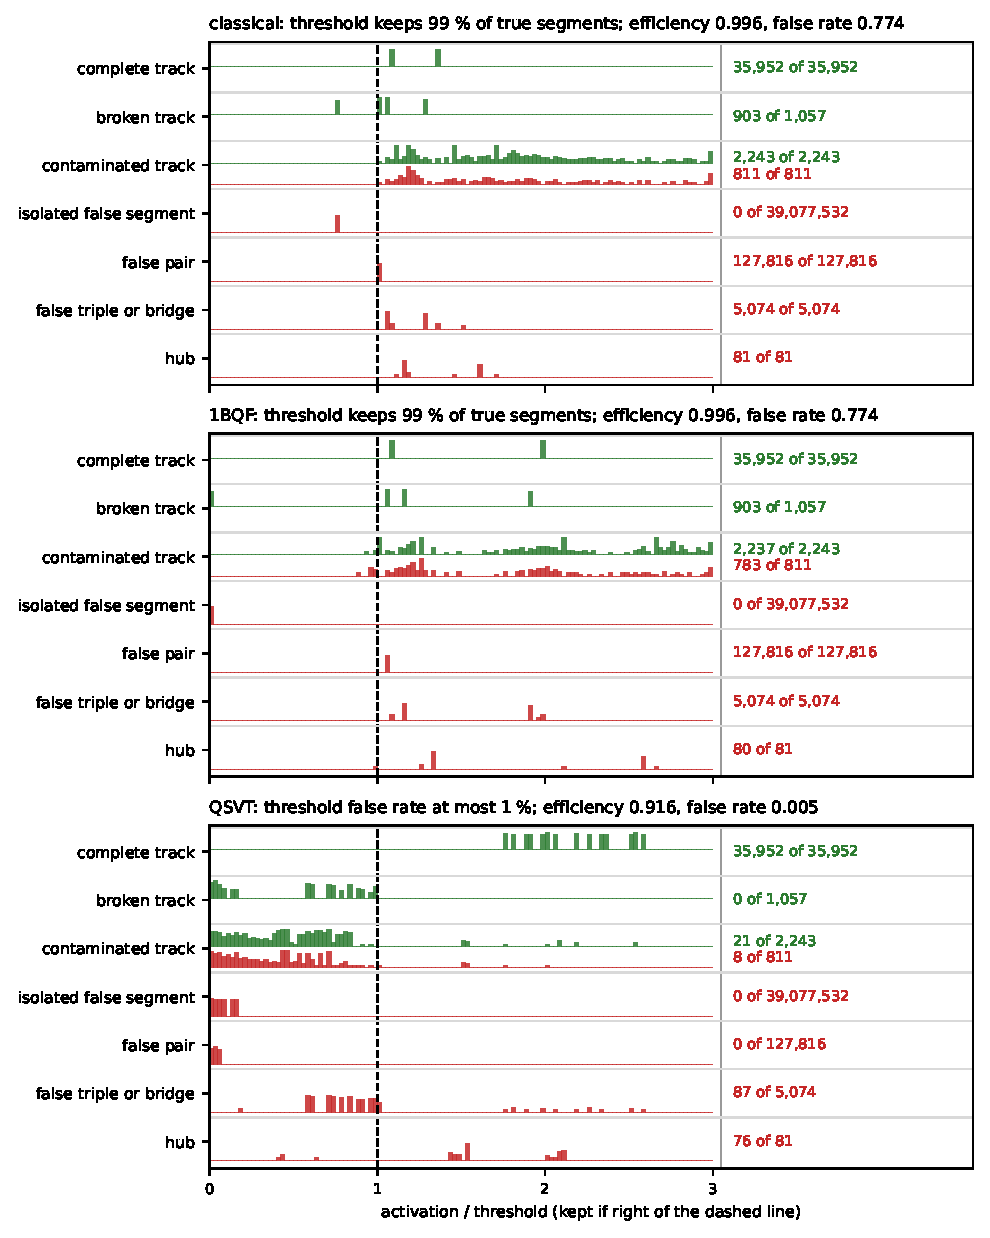
\includegraphics[width=0.92\textwidth]{fig3_error_atlas_T1000_with_qsvt.pdf}
\caption{\textbf{What each solver keeps}, by kind of group, at 1000 tracks pooled over
$\NEvents$ events. Activations are divided by each solver's threshold, so a segment is kept
when it lies to the right of the dashed line. Green, true segments; red, false; the kept
counts are given on the right. Classical solver and one-bit filter: threshold keeping $99\%$ of
true segments. Polynomial: lowest threshold with a false rate of at most $1\%$ \js{how is false rate defined? Because for the classical solver, it filters out nearly 40,000,000 tracks, right?} \gs{The false rate is the number of false segments kept divided by the number of all segments kept. It is one minus the purity. It is not the fraction of the 39 million candidates that leak. We will define it at the first use.}. The same figure at 400 tracks is in the supplement. \js{what is classical solver? Can you give a reference please?} \gs{The classical solver is the direct solution of $A\mathbf{x}=\mathbf{b}$, read at a threshold on $x_i$, as in refs.~\cite{nicotra2023,trackhhl}. We will define it and cite it at the first use.}}
\label{fig:atlas}
\end{figure}

\begin{table}[t]
\centering\small
\caption{False rate at $99\%$ efficiency for the classical solver and the one-bit filter, and
efficiency at a false rate of at most $1\%$ for the polynomial, as medians over $\NEvents$ events
(lowest event in brackets). \js{Why is the line between two efficiencies? And why is there no polynomial: false rate at 99\% efficiency? } \gs{The line separates the working points we use (first three rows) from the two cross-check rows. We will replace it by a clearer layout. The missing row exists: the median false rate of the polynomial at $99\%$ efficiency is $0.56$ at 200 tracks, $0.36$ at 400, $1.00$ at 700 and $1.00$ at 1000. To keep $99\%$ of true segments the threshold must reach the broken tracks, and the rejected population lies at the same level. We will add this row and this sentence.}}
\label{tab:headline}
\begin{tabular}{lcccc}\toprule
 & $T=200$ & $T=400$ & $T=700$ & $T=1000$\\\midrule
Classical: false rate at $99\%$ efficiency & $\ClassFarTwoHundred$ & $\ClassFarFourHundred$ & $\ClassFarSevenHundred$ & $\ClassFarThousand$\\
One-bit filter: false rate at $99\%$ efficiency & $\OneBitFarTwoHundred$ & $\OneBitFarFourHundred$ & $\OneBitFarSevenHundred$ & $\OneBitFarThousand$\\
Polynomial: efficiency at false rate $\le1\%$ & $\QsvtEffTwoHundred$ ($\QsvtEffMinTwoHundred$) & $\QsvtEffFourHundred$ ($\QsvtEffMinFourHundred$) & $\QsvtEffSevenHundred$ ($\QsvtEffMinSevenHundred$) & $\QsvtEffThousand$ ($\QsvtEffMinThousand$)\\
\midrule
One-bit filter: efficiency at false rate $\le1\%$ & $\OneBitEffAtOneTwoHundred$ & $\OneBitEffAtOneFourHundred$ & $\OneBitEffAtOneSevenHundred$ & $\OneBitEffAtOneThousand$\\
Classical: efficiency at false rate $\le1\%$ & $\ClassEffAtOneTwoHundred$ & $\ClassEffAtOneFourHundred$ & $\ClassEffAtOneSevenHundred$ & $\ClassEffAtOneThousand$\\\bottomrule
\end{tabular}
\end{table}

\paragraph{The one change. \js{not a very scientific title} \gs{We will rename the paragraph `A response with more than one zero'.}} Every kind of group in figure~\ref{fig:atlas} sits on eigenvalues that are fixed by its graph, so
separating them does not need a different primitive, only a response with more than one zero.
The quantum singular value transformation provides it: $d$ calls to a block encoding of $A$,
with a phase rotation between calls, apply any polynomial of degree $d$ bounded by 1 on $[-1,1]$
(figure~\ref{fig:filters}b). Section~\ref{sec:r2} shows where the eigenvalues of each kind lie,
what the transformation is, and which polynomial we apply; section~\ref{sec:r3} measures it against
track multiplicity.

%==============================================================================================
\subsection{The problem as a spectrum, and a polynomial that separates it}\label{sec:r2}

\paragraph{Every block has a spectrum fixed by its graph.}
\js{I think that this should come prior to here} \gs{Agreed, see our reply at the Hamiltonian paragraph. This paragraph moves to section~\ref{sec:r1}.}
Because $A=\lambda_cI-C$ is block-diagonal, its eigenvalues are those of the individual blocks, and
on a block of $m$ segments with compatibility graph $G$ they are
\begin{equation}
\lambda=\lambda_c-\mu,\qquad \mu\in\operatorname{spec}\big(C_G\big),
\end{equation}
where $C_G$ is the adjacency matrix of $G$. The graphs that occur are small and their spectra are
known in closed form. A chain of $m$ segments, which is what a complete track ($m=4$) or a broken
track ($m\le3$) is, has
\begin{equation}
\lambda_k=\lambda_c-2\cos\!\Big(\frac{k\pi}{m+1}\Big),\qquad k=1,\dots,m ,
\end{equation}
so a complete track owns exactly four eigenvalues, $\{2.382,\,3.382,\,4.618,\,5.618\}$ at
$\lambda_c=4$. An isolated segment has the single eigenvalue $\lambda_c$; a pair of compatible
segments has $\lambda_c\mp1$; a triple has $\lambda_c$ and $\lambda_c\mp\sqrt2$; and a hub, in which
$m$ segments leave or enter one hit, has $\lambda_c\pm\sqrt m$ together with $m-1$ copies of
$\lambda_c$. None of these depends on the event: detector geometry fixes the graph of a complete
track, and hence its four lines, for every track in every event.

\paragraph{Only some lines carry weight.}
The solution to \eqref{eq:Axb} on a block is a sum over its eigenvectors $\mathbf{v}_k$,
\begin{equation}
\mathbf{x}\big|_{\rm block}=\sum_k\frac{\langle\mathbf{v}_k,\mathbf{b}\rangle}{\lambda_k}\,\mathbf{v}_k ,
\end{equation}
and the uniform input $\mathbf{b}=\beta\mathbf{1}$ reaches only the modes that are symmetric under
every relabelling of the block that leaves its graph unchanged; every other mode has
$\langle\mathbf{v}_k,\mathbf{b}\rangle=0$ exactly \js{I do not understand this} \gs{The input $\mathbf{b}=\beta\mathbf{1}$ is the same on every segment. A relabelling of the segments that keeps the graph is a permutation $P$ with $PCP^{\mathsf T}=C$ and $P\mathbf{1}=\mathbf{1}$. For an eigenvector with $P\mathbf{v}=-\mathbf{v}$ we get $\langle\mathbf{v},\mathbf{1}\rangle=\langle P\mathbf{v},P\mathbf{1}\rangle=-\langle\mathbf{v},\mathbf{1}\rangle$, so the overlap is zero. For the chain, $P$ is the reflection and the modes $v_j=\sin(kj\pi/(m+1))$ with even $k$ are antisymmetric. We will add this argument.}. We call a mode bright when that overlap is non-zero and
dark when it vanishes. A dark mode has an eigenvalue but no amplitude \js{??} \gs{Meaning: the eigenvalue is in the spectrum of the block, but the input vector has zero component along that eigenvector. A function $g(A)$ multiplies each eigencomponent by the scalar $g(\lambda_k)$, so a zero component stays zero. We will rewrite the sentence.}, and no function of $A$ applied
to $\mathbf{b}$ can give it one. For a chain the reflection $j\mapsto m+1-j$ is the only such
relabelling, so its antisymmetric modes are dark: a complete track is bright only on $2.382$ and
$4.618$, and carries $\TrackInputWeightLow\%$ of its input weight on the first
($\TrackSolutionWeightLow\%$ of its solution). A pair is bright only on $\lambda_c-1$, a triple on
$\lambda_c\mp\sqrt2$, and a hub of any size only on $\lambda_c\pm\sqrt m$. \js{I would need more explanation on this whole paragraph I guess.} \gs{We will expand this paragraph with the argument above and with the explicit chain eigenvectors.}

\paragraph{What noise does to the spectrum.}
Figure~\ref{fig:spectrum}a shows where the input weight actually lands on the corpus at 1000 tracks,
split by kind of group. Complete tracks put all of their weight on their two bright lines, and
$\NIsolatedThousand$ isolated segments sit exactly at $\lambda_c$. The false pairs sit on
$\lambda_c-1=3$, the false triples on $\lambda_c\mp\sqrt2$, and the broken tracks on the lines of
their shorter chains; all of them lie between the true lines, not on them. Two kinds are harder.
A hub with three prongs has its bright line at $\lambda_c-\sqrt3=2.268$, only $0.11$ from the
track line at $2.382$, and $\HubNearTrue\%$ of the hubs' weight falls within $0.18$ of a bright true
line. A contaminated track, a real track that carries an accidental false segment, is no longer a
chain: its graph is a tree, its lines move, and only $\ContamNearTrue\%$ of its weight stays near
the true lines. These two kinds set the limits of every filter that acts on the spectrum alone.

\paragraph{The one-bit filter, read on the spectrum.}
Figure~\ref{fig:spectrum}b places the one-bit response $|\cos(\lambda t/2)|$ on the same axis. Its
single zero sits on the line that carries the most segments, $\lambda_c$, and removes them. On every
other line its factor is set by the distance from $\lambda_c$ alone, which is why the false pair at
$\lambda_c-1$ keeps $\KeptPair$, less than the track line at $2.382$ ($\KeptTrack$) only because it is
closer to the zero, and why the hub line at $2.268$, further from the zero than the track line,
keeps more ($\KeptHubThree$). A single cosine cannot be low on $3$ and high on $2.382$ without also
being high on $2.268$ and $2.586$: its shape is fixed, and only its zero can be placed.

\begin{figure}[p]
\centering
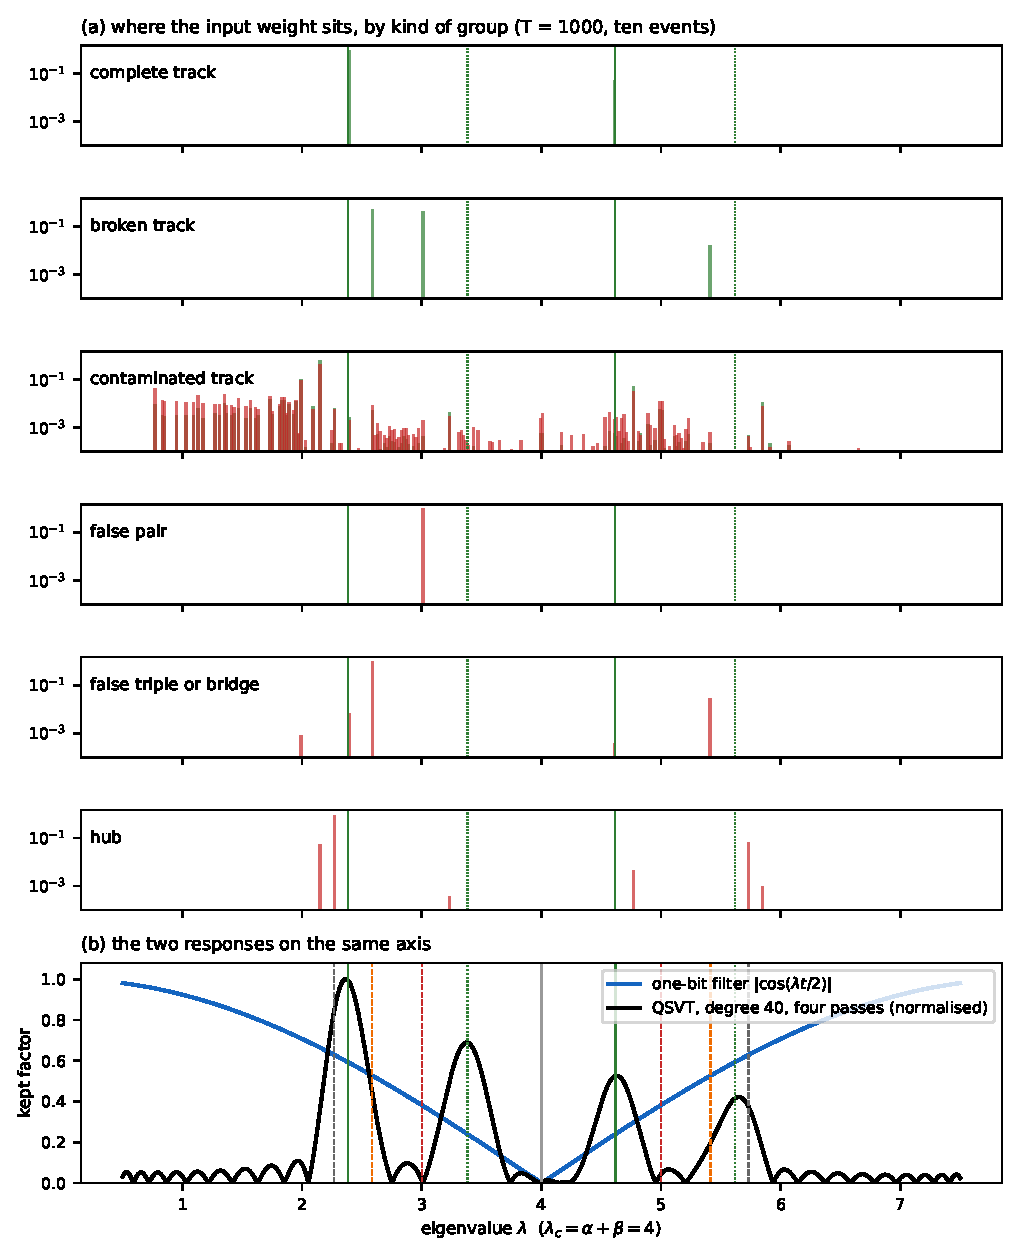
\includegraphics[width=0.92\textwidth]{fig4_spectrum.pdf}
\caption{\textbf{The problem as a spectrum.} (a)~Bright weight $\langle\mathbf{v}_k,\mathbf{1}\rangle^2$ of
every eigenmode, by kind of group, on ten events with 1000 tracks; green, weight on true segments;
red, on false segments; each lane normalised to its total. The isolated segments, all at
$\lambda_c=4$, are not drawn. Vertical lines: the four lines of a complete track (solid, bright;
dotted, dark). (b)~The one-bit filter $|\cos(\lambda t/2)|$ and the QSVT polynomial (degree 40, four
passes \js{passes = ?} \gs{A pass is an interval of the eigenvalue axis where the response is near its maximum. The target function has one pass on each of the four lines of a complete track. We will define `pass' at its first use in section~\ref{sec:r2}.}, normalised to its maximum) on the same axis; dashed lines mark the pair ($\lambda_c\mp1$,
red), triple ($\lambda_c\mp\sqrt2$, orange) and three-prong hub ($\lambda_c\pm\sqrt3$, grey)
eigenvalues.}
\label{fig:spectrum}
\end{figure}

\paragraph{Block encodings and the quantum singular value transformation.}
A quantum circuit cannot apply $A$ directly, because $A$ is not unitary. It can apply a unitary $U$
that contains a rescaled copy of $A$ in one corner. With $X=(A-c_0I)/c_1$ \js{How do we choose $c_0$ and $c_1$? We should shortly comment on that I guess already here.} \gs{$c_0$ is the centre and $c_1$ the half-width of the fit interval $[\lambda_{\min}-\Delta,\lambda_{\max}+\Delta]$ of the paragraph on the polynomial. $\lambda_{\min}$ and $\lambda_{\max}$ are the extreme eigenvalues of the event, computed by the Lanczos method. We will define $c_0$ and $c_1$ here.} chosen so that the spectrum
of $X$ lies in $[-1,1]$, a block encoding of $X$ is a unitary on the segment register and one or more
ancilla qubits with
\begin{equation}
\big(\langle0|\otimes I\big)\,U\,\big(|0\rangle\otimes I\big)=X .
\end{equation}
The simplest one, used in figure~\ref{fig:filters}b and in our simulations, is the dilation
\begin{equation}
U=\begin{pmatrix}X&\sqrt{I-X^2}\\ \sqrt{I-X^2}&-X\end{pmatrix},
\end{equation}
which needs a single ancilla; a construction that prices each call by detector hits rather than by
matrix entries is discussed in section~\ref{sec:r5} \js{Not sure this is needed here already. The paper is heavy enough as it is.} \gs{Agreed. We will remove the forward reference and keep the hit-priced block encoding for section~\ref{sec:r5} only.}. The quantum singular value
transformation~\cite{gslw2019,martyn2021} then states that for every real polynomial $p$ of degree
$d$ with definite parity and $|p(x)|\le1$ on $[-1,1]$ there exist phases $\phi_0,\dots,\phi_d$ such
that the circuit
\begin{equation}
U_\Phi=e^{i\phi_0(2\Pi-I)}\prod_{k=1}^{d}\Big[U^{(\dagger)}\,e^{i\phi_k(2\Pi-I)}\Big],\qquad \Pi=|0\rangle\langle0|\otimes I,
\end{equation}
with $U$ and $U^\dagger$ alternating, has in the same corner a polynomial $P(X)$ whose real part is
$p(X)$. It makes $d$ calls in total, to $U$ and $U^\dagger$ in alternation, \js{Should this not be $U$ and $U^\dagger$ in total $d$ times?} \gs{Yes. Corrected: the sequence makes $d$ calls in total, to $U$ and $U^\dagger$ in alternation.}
and adds one signal qubit for the phases, and the phases are computed classically once for a given
$p$~\cite{dong2021}. A polynomial without definite parity is split into its even and odd parts, each
realised by its own phase sequence and combined with one further ancilla; the real part of the
complex polynomial the sequence produces is selected the same way. Measuring the ancillas in
$|0\rangle$ leaves the segment register in the state $p(X)|u\rangle/\lVert p(X)|u\rangle\rVert$, with
probability $\lVert p(X)|u\rangle\rVert^2$ up to a constant factor from the ancillas that select the
real part and combine the parities, where $|u\rangle$ is the uniform superposition over segments. Equivalently, since $\langle0|W^k|0\rangle=T_k(X)$ for the qubitised walk $W=(Z\otimes I)U$
built from the dilation~\cite{lowchuang2019}, a polynomial written as a Chebyshev series
$p(X)=\sum_kc_kT_k(X)$ can be applied as a linear combination of walk powers~\cite{childs2012}, at the
price of $\lceil\log_2(d+1)\rceil$ index qubits and a success probability reduced by
$(\sum_k|c_k|)^2$. Both routes apply the same polynomial; which is cheaper is the subject of
section~\ref{sec:r4}.

\paragraph{The one-bit filter is the degree-one case.}
The one-bit filter uses no block encoding: it calls the controlled evolution $e^{-iAt}$ directly.
The same polynomial construction applies to controlled evolutions~\cite{dong2022}, with the
variable $u=\cos(\lambda t/2)$ in place of $x$: a sequence of $d$ controlled evolutions with phase
rotations between them applies polynomials of degree $d$ in $u$ bounded by 1 on $[-1,1]$, subject to the same parity
conditions. The one-bit
interferometer is the shortest such sequence, and the response it applies, $\cos(\lambda t/2)$, is
the polynomial $p(u)=u$: degree one, one root. Every further call buys one further degree, and with
it one further zero or pass that can be placed on the spectrum. \js{I think that this paragraph is very important, so it deserves a bit more details, right? Can we see directly from Fig. 2a and b that the statement is true? Or can we compute it based on the exact representation of the final result of the algorithms?} \gs{Yes, we can compute it from the circuit. In figure~\ref{fig:filters}a the two Hadamard gates around the controlled $e^{-iAt}$ give, on the $T=0$ part, $\tfrac12(I+e^{-iAt})=e^{-iAt/2}\cos(At/2)$. This is a block encoding of $\cos(At/2)$ up to a phase. It is the degree-one case of the construction of ref.~\cite{dong2022}, with the controlled evolution in place of $U$. Figure~\ref{fig:filters}b with $d=1$ and this $U$ is the same circuit. We will add this derivation to the paragraph.} 

\paragraph{The polynomial we apply.}
The spectrum of figure~\ref{fig:spectrum}a tells us what the response should do: pass the lines of a
complete track and reject everything between them. We write this as a target function on the
eigenvalue axis,
\begin{equation}
g(\lambda)=\frac{1}{\lambda}\max_{k}\exp\!\Big[-\Big(\frac{\lambda-\lambda_k}{h}\Big)^2\Big],\qquad
\lambda_k=\lambda_c-2\cos\!\Big(\frac{k\pi}{5}\Big),
\end{equation}
a narrow pass of half-width $h$ \js{$h$ defined as ...?} \gs{$h$ is the half-width of each pass in eigenvalue units, $h=0.18$ throughout. The sentence will say `where $h$ is the half-width of each pass'.} on each true line, weighted by $1/\lambda$ so that on those lines
the response keeps the relative amplitudes of the classical solution. We fit $g$ by least squares
with a Chebyshev series of degree $d$ on the interval $[\lambda_{\min}-\Delta,\lambda_{\max}+\Delta]$,
where $\lambda_{\min}$ and $\lambda_{\max}$ are bounds on the spectrum of the event and
$\Delta=0.05(\lambda_{\max}-\lambda_{\min})+0.2$ a margin, and rescale the result so that
$|p|\le0.95$ on the interval \js{I guess you mean the interval from $\lambda_{\min}$ to $\lambda_{\max}$? Then specify it. } \gs{No, the fit interval $[\lambda_{\min}-\Delta,\lambda_{\max}+\Delta]$. The bound must hold on the full domain of the block encoding, and this domain is the fit interval. We will name it.}. Throughout this paper $d=40$ and $h=0.18$, and we call this
polynomial the QSVT.

\paragraph{Why degree 40.}
A polynomial of degree $d$ on an interval of half-width $W$ \js{Is there a reason not to go with the full width? Then you save all these factors of two.} \gs{No reason. We will use the full width $L=2W$ and write the resolution as $L/d$.} cannot resolve features narrower than
about $2W/d$ \js{This is so unspecific, that it is meaningless. What does 'features' mean? If you mean roots, then this makes sense} \gs{Agreed. A polynomial of degree $d$ has at most $d$ zeros, so the mean distance between adjacent zeros on an interval of length $L$ is at least $L/d$. A pass or a notch needs two zeros around it, so it cannot be narrower than this distance. We will write it in this way.}. At 1000 tracks the interval is $[\DomainLow,\DomainHigh]$, so $W=\DomainHalfWidth$ and
degree 40 resolves $\ResolutionForty$, degree 60 $\ResolutionSixty$. The closest false line the design aims to reject is the triple line at $2.586$, $0.20$ from the
track line at $2.382$, which degree 40 just resolves; the three-prong hub line at $2.268$, $0.11$ away,
is beyond it. The resulting response (figure~\ref{fig:spectrum}b) keeps
$\QTrackLow$ of its maximum on the dominant track line and $\QTrackHigh$ on the second, and
$\QPairLow$ on the false pair line, against $\KeptPair$ for the one-bit filter: relative to the
track line, the false pairs, the largest coupled false population, are suppressed
$\PairSuppression$ \js{If I compute correctly, 0.38/0.014 = 27, so not 45. Or am I mistaken?} \gs{The ratio 27 is the absolute ratio of the two pair factors. The value 45 is relative to the track line, as the sentence says: $(\KeptPair/\KeptTrack)/(\QPairLow/\QTrackLow)=45.8$. We will write this formula in the text so that the reader can check it.} times more strongly than by the one-bit filter. It keeps $\QIso$ on the isolated line, not zero, but on so small a factor that isolated
segments fall far below every true track. It keeps $\QTripleLow$ on the triple line at $2.586$,
which sits on the flank of the track pass, and $\QHubLow$ on the hub line at $2.268$, which no
polynomial of this degree can separate from the track line $0.11$ away.

\paragraph{Two passes or four.}
\js{Again, you should explain what you mean by passes!} \gs{See our reply at figure~\ref{fig:spectrum}. We will define `pass' in section~\ref{sec:r2} before this point.}
A complete track is bright only on two of its four lines, so passes on the two dark lines might
seem wasted. We tested this directly on the corpus \js{Funny, but not scientifically ;-)} \gs{We will replace `directly on the corpus' by `on the simulated events of section~\ref{sec:r1}'.} with $\TeethNDesigns$ designs (four passes or two
bright passes, degrees 24, 40 and 60, half-widths $0.12$ to $0.30$), choosing on five events and
measuring on the other five. Placing the passes on the two dark lines alone destroys the filter:
efficiency at a false rate of at most $1\%$ falls to $\TeethDarkTwoHundred$ at 200 tracks and
$\TeethDarkThousand$ \js{Really exactly zero?} \gs{The median over the five held-out events is exactly zero. The largest value on one event is $0.0005$. We will write `below $0.001$ on every held-out event'.} at 1000, a direct confirmation that tracks live on their bright lines. At equal
degree and width, two bright passes and four passes give the same result within the event-to-event
spread ($\TeethBrightThousand$ against $\TeethFourThousand$ at 1000 tracks, degree 40); the
advantage that bright passes alone showed on noiseless events in our earlier study does not carry
over to these events. What does matter is resolution. Degree 60 with half-width $0.12$ raises the efficiency at 700 tracks from
$\TeethFourSeven$ to $\TeethFourSixtySeven$ with four passes and to $\TeethBestSeven$ with two, and at
1000 tracks to $\TeethFourSixtyThousand$ and $\TeethBestThousand$, at one and a half times the calls.
We keep degree 40 with four passes as the reference design and report the higher degree as a variant
in section~\ref{sec:r3}.

\paragraph{Reading the output.}
After post-selection the probability of reading segment $i$ is proportional to
$[p(A)\mathbf{b}]_i^2$, so the amplitude $|[p(A)\mathbf{b}]_i|$ plays the role that $x_i$ plays for
the classical solver. Its distribution separates sharply: the segments of complete tracks sit well above
everything the polynomial rejects, with broken tracks, contaminated tracks and false triples in
between (figure~\ref{fig:atlas}).
We therefore read the QSVT at the lowest threshold with a false rate of at most $1\%$ and report the
efficiency it keeps, while the classical solver and the one-bit filter, whose true and false levels overlap, are read at the threshold that keeps $99\%$ of true segments. In all our figures the QSVT
amplitudes are computed exactly, by applying $p$ to the eigenvalues of each block and checked
against the three-term Chebyshev recursion on the full sparse matrix; they are what any exact
realisation of the circuit produces after post-selection.

%==============================================================================================
\subsection{Results against track multiplicity}\label{sec:r3}
\textit{[To be drafted: efficiency and false rate against $T$ for all three solvers, the degree-60
variant, full efficiency--false-rate curves.]}

\subsection{Computational cost}\label{sec:r4}
\textit{[To be drafted: width, calls, gates per call, amplification, readout; HHL, one-bit filter and
QSVT in one currency.]}

\subsection{A block encoding priced by detector hits}\label{sec:r5}
\textit{[Scope to be decided: cost model here, construction possibly in a separate paper.]}

\clearpage
\section*{\textit{Discussion and Methods: to be drafted}}

\begin{thebibliography}{99}
\bibitem{denby1988} B.~Denby, \emph{Neural networks and cellular automata in experimental high energy physics}, Comput.\ Phys.\ Commun.\ \textbf{49} (1988) 429.
\bibitem{peterson1989} C.~Peterson, \emph{Track finding with neural networks}, Nucl.\ Instrum.\ Meth.\ A \textbf{279} (1989) 537.
\bibitem{hhl2009} A.~W.~Harrow, A.~Hassidim and S.~Lloyd, \emph{Quantum algorithm for linear systems of equations}, Phys.\ Rev.\ Lett.\ \textbf{103} (2009) 150502.
\bibitem{nicotra2023} D.~Nicotra et al., \emph{A quantum algorithm for track reconstruction in the LHCb vertex detector}, JINST \textbf{18} (2023) P11028.
\bibitem{trackhhl_epj} X.~Chiotopoulos, M.~L.~Martinez, D.~Nicotra, J.~A.~de~Vries, K.~Driessens, M.~Merk and M.~H.~Winands, \emph{TrackHHL: A Quantum Computing Algorithm for Track Reconstruction at the LHCb}, EPJ Web Conf.\ \textbf{337} (2025) 01181; arXiv:2511.11458.
\bibitem{trackhhl} X.~Chiotopoulos, D.~Nicotra, G.~Scriven, K.~Driessens, M.~Merk, J.~Sch\"utz, J.~de~Vries and M.~H.~M.~Winands, \emph{A 1-bit quantum filter for particle trajectory reconstruction}, Commun.\ Phys.\ (2026), doi:10.1038/s42005-026-02780-8; arXiv:2601.07766.
\bibitem{gslw2019} A.~Gily\'en, Y.~Su, G.~H.~Low and N.~Wiebe, \emph{Quantum singular value transformation and beyond: exponential improvements for quantum matrix arithmetics}, Proc.\ 51st ACM STOC (2019) 193; arXiv:1806.01838.
\bibitem{lowchuang2019} G.~H.~Low and I.~L.~Chuang, \emph{Hamiltonian simulation by qubitization}, Quantum \textbf{3} (2019) 163.
\bibitem{childs2012} A.~M.~Childs and N.~Wiebe, \emph{Hamiltonian simulation using linear combinations of unitary operations}, Quantum Inf.\ Comput.\ \textbf{12} (2012) 901.
\bibitem{dong2021} Y.~Dong, X.~Meng, K.~B.~Whaley and L.~Lin, \emph{Efficient phase-factor evaluation in quantum signal processing}, Phys.\ Rev.\ A \textbf{103} (2021) 042419; arXiv:2002.11649.
\bibitem{dong2022} Y.~Dong, L.~Lin and Y.~Tong, \emph{Ground-state preparation and energy estimation on early fault-tolerant quantum computers via quantum eigenvalue transformation of unitary matrices}, PRX Quantum \textbf{3} (2022) 040305; arXiv:2204.05955.
\bibitem{martyn2021} J.~M.~Martyn, Z.~M.~Rossi, A.~K.~Tan and I.~L.~Chuang, \emph{Grand unification of quantum algorithms}, PRX Quantum \textbf{2} (2021) 040203.
\end{thebibliography}
\end{document}
